\section{Dossier de spécifications}

\par À l’issue de la première réunion avec Mr Stéphane Vialle, cahier des charges, déroulement du projet, éventuelles difficultés et objectif du projet développement ont été établis. Il est important de rappeler l'objectif d'un tel projet académiquement parlant. Il s'agit pour les élèves d'apprendre à :

\begin{itemize}
\item formaliser un cahier des charges;
\item décrire un projet sous forme UML (diagramme de classe, séquence, \emph{use case});
\item réaliser un plan de test;
\item réaliser une documentation (\emph{user guide}) et une architecture logicielle;
\item coder une interface graphique contenant de l’héritage;
\item travailler sur des fichiers I/O.
\end{itemize}

\par L’architecture générale du projet est donnée à la figure~\ref{fig:schema_global} ci-dessous. L’idée est d’agréger une couche logicielle à l’environnement \emph{OAR}, évitant ainsi l'allocation de noeuds via des commandes \emph{shell}.  Pour de plus amples informations sur \emph{OAR} et les commandes \emph{shell} nécessaires afin de se connecter et d’allouer des nœuds de calcul, vous vous référerez à la partie \ref{sec:oar-gestionnaire-res}.

\par Le but principal est d’allouer des nœuds et de récupérer un fichier .txt contenant la description détaillée des noeuds alloués. À savoir les machines allouées, leur noms, la date et l'heure d'allocation, la fin d'allocation, l'identifiant du job, et bien d'autres. Ce fichier devra être présenté à l'utilisateur, lorsque celui-ci en fait la demande, et mis à jour à chaque modification du job.
\begin{figure}[h!]
  \centering
  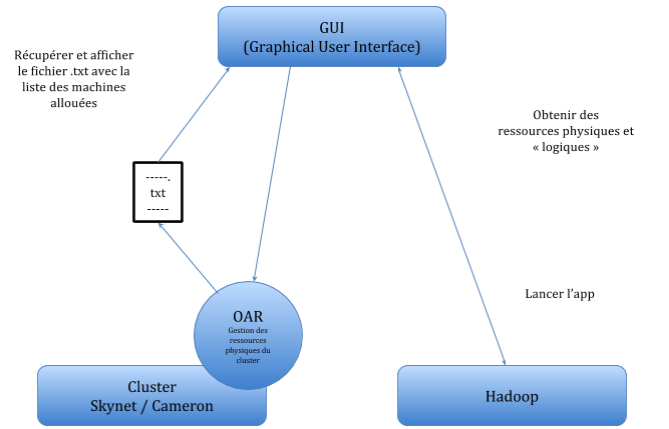
\includegraphics[width=14cm]{images/schema_global.png}
  \caption{Schéma global de fonctionnement de l'application}
  \label{fig:schema_global}
\end{figure}

\par Pour la deuxième partie du projet au cours de la séquence 8, nous utiliserons cette GUI (en anglais \emph{Graphic User Interface}) afin de lancer des applications Hadoop. Pour de plus amples explications concernant l'environnement Hadoop, vous vous référerez au rapport le traitant.
\par Par ailleurs, toutes les requêtes auprès des clusters de Supélec nécessitent des accès sur nos comptes. Accès dont nous avons bénéficié pour nous familiariser avec \emph{OAR}.

\subsection{Architecture du serveur de Supélec}
\label{sec:archi-serveur-supelec}

\par Avant toute chose, il est indispensable de comprendre l'architecture des serveurs de Supélec. Ce serveur est composé de deux machines frontales : \emph{ghome} et \emph{term2} (pour \emph{Terminator 2}). La figure \ref{fig:archi_serveur} reprend cette architecture. Tout utilisateur ayant les droits d'accès au serveur doit impérativement se connecter à la machine \emph{ghome} avant de connecter à \emph{term2} à travers laquelle il pourra allouer des noeuds grâce à l'environnement \emph{OAR} au sein des clusters \emph{Skynet}, \emph{Cameron} et \emph{InterCel}. Cependant, si l'utilisateur est connecté au réseau de Supélec, l'identification auprès de \emph{term2} est suffisante. Dans le cas échéant il devra nécessairement passer par \emph{ghome}.
\par À titre d'information, \emph{OAR} gère aussi les ressources du cluster \emph{Scooby}. Ce cluster n'est pas utilisé au cours de notre projet.

\begin{figure}[h!]
  \centering
  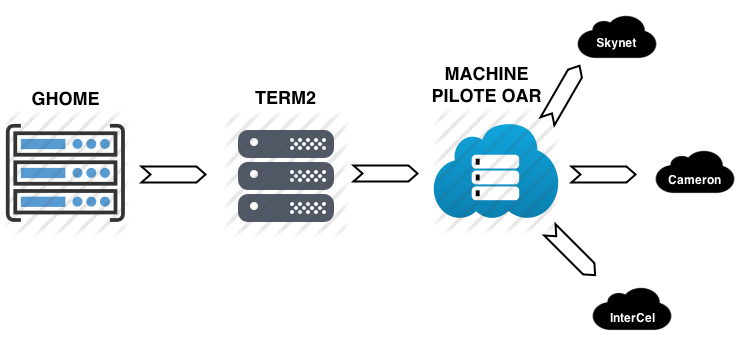
\includegraphics[width=14cm]{images/archi_serveur_supelec.png}
  \caption{Architecture des serveurs de Supélec}
  \label{fig:archi_serveur}
\end{figure}

\subsection{Le diagramme \emph{use case}}
\label{sec:le-diagramme-use}

\par La figure \ref{fig:use_case} donne le diagramme \emph{use case} du projet. Plusieurs scénarios peuvent être répertoriés :

\begin{itemize}
\item \emph{S’identifier};
\item \emph{Créer un job (Allocation de nœuds)};
\item \emph{Tuer le job};
\item \emph{Exécuter des codes Hadoop};
\end{itemize}

\begin{figure}[h!]
  \centering
  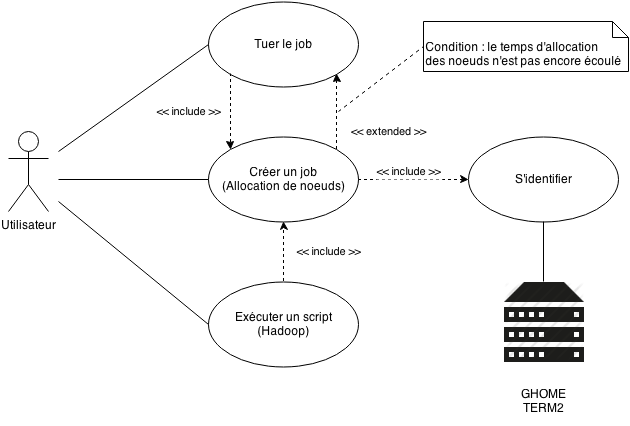
\includegraphics[width=14cm]{images/use_case.png}
  \caption{Use case}
  \label{fig:use_case}
\end{figure}

\paragraph{Scénario \emph{«S’identifier»}}
\par Compte tenu des remarques du paragraphe \ref{sec:le-diagramme-use}, il est à rajouter que l'identification préalable auprès de \emph{ghome} n'étant pas gênant pour la suite de l'identification bien que ce dernier soit connecter au réseau de Supélec, nous avons décidé, par souci de praticité, de toujours identifier l'utilisateur auprès de \emph{ghome} puis de \emph{term2}.
\par Cette étape consiste à vérifier la validité du nom ainsi que du mot de passe de l’utilisateur.

\paragraph{Scénario \emph{«Créer un job (Allocation de nœuds)»}}
\label{sec:scenario-creer-un}
\par Après identification, l’utilisateur sera en mesure de créer un job, i.e. d’allouer des nœuds de calcul. Il renseignera donc le nombre de nœuds et le temps d’allocation souhaités. Deux cas de figure se présentent à l'utilisateur. Après la création d’un job, si le temps d’allocation est écoulé le job est automatiquement tué. Dans le cas contraire, l’utilisateur pourra interagir avec la GUI afin de renouveler son job en mettant fin au précédent.

\paragraph{Scénario \emph{«Tuer le job»}}
\label{sec:scenario-tuer-le}
\par Ce scénario n’est évidemment possible que lorsqu’un job a été au préalable créé et que l’utilisateur est connecté au serveur. 

\paragraph{Scénario \emph{«Exécuter un script (Hadoop)»}}
\label{sec:scenario-executer-un}
\par Ce scénario sera abordé dans la deuxième partie du projet se déroulant au cours de la séquence 8.


\subsection{Cahier des charges}
\label{sec:cahier-des-charges}

\par Trois grandes parties composent le cahier des charges.

\subsubsection{Points essentiels}
\label{sec:points-essentiels}

\par La phase d'analyse des différents scénarios a permis d'aboutir à trois points essentiels pour le projet. D’abord nous créerons une IU (Interface Utilisateur) de connexion aux serveurs à travers laquelle il sera possible de spécifier le nom de la machine, le nom de l'utilisateur et son mot de passe.
Ensuite, on créera une deuxième IU d’allocation des nœuds ou seront spécifiés le nombre de nœuds, leur temps d’allocation ainsi que le mode d’allocation (on choisit par défaut le mode interactif).
Enfin, un fichier .txt contenant la description des nœuds alloués devra être récupéré.

\begin{figure}[h!]
  \centering
  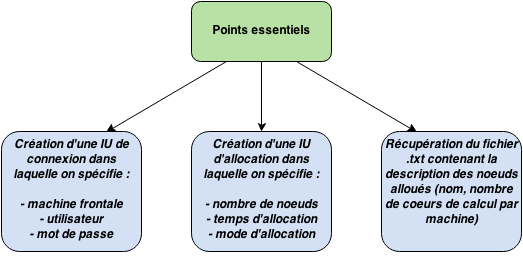
\includegraphics[width=12cm]{images/points_essentiels.png}
  \caption{Cahier des charges : les points essentiels}
  \label{fig:pts_essentiels}
\end{figure}


\subsubsection{Points souhaités}
\label{sec:points-souhaites}

\par Parmi les options fortement souhaitées, l’IU d’allocation devra comporter une zone de texte où sera affiché le temps d’allocation des nœuds en temps réel ainsi que les noms des machines allouées. En outre, le fichier .txt devra être redirigé vers cette zone de texte.

\begin{figure}[h!]
  \centering
  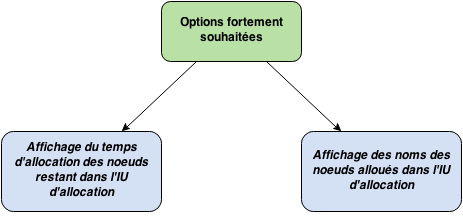
\includegraphics[width=11cm]{images/points_souhaites.png}
  \caption{Cahier des charges : les options fortement souhaitées}
  \label{fig:pts_souhaites}
\end{figure}

\subsubsection{Points optionnels}
\label{sec:points-optionnels}

\par Nous avons retenu trois développements optionnels. Leur réalisation est conditionnée par l’état d’avancement du projet (priorité aux points essentiels et aux options fortement souhaitées) et de leur faisabilité technique.
\par Le premier consiste à obtenir un état des lieux du serveur, i.e. à recenser les ressources physiques disponibles lors de la connexion. L’idée étant dans une deuxième partie de donner à l’utilisateur la possibilité de choisir entre les différents clusters les machines avec lesquelles il désire travailler. En effet, selon que l’on se trouve sur le cluster Skynet, Cameron ou InterCel, les machines ne possèdent pas les mêmes puissances de calcul.
\par Troisièmement, dans le souci de rendre l’expérience utilisateur la plus agréable possible, un design épuré serait fort appréciable. Bien entendu, ce point sera abordé uniquement si tous les précédents points ont été réalisés et validés les tests.

\begin{figure}[h!]
  \centering
  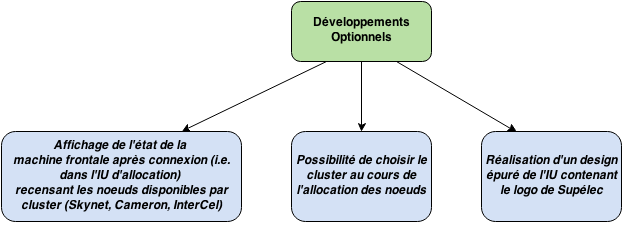
\includegraphics[width=14cm]{images/points_optionnels.png}
  \caption{Cahier des charges : les développements optionnels}
  \label{fig:pts_optionnels}
\end{figure}



%%% Local Variables: 
%%% mode: latex
%%% TeX-master: "CompteRendu"
%%% End: 
